\documentclass{article}
\usepackage{xeCJK}
\usepackage{ctex}
\usepackage{indentfirst}
\usepackage{graphicx}
\usepackage{caption}
\usepackage{subcaption}
\usepackage{geometry}
\usepackage{listings}
\usepackage{xcolor}
\usepackage{amsmath}
\usepackage{multicol} %用于实现在同一页中实现不同的分栏

\graphicspath{{./image/}}
\setlength{\parindent}{2em}
\geometry{a4paper,scale=0.9}
\lstset{
    basicstyle          =   \sffamily,          % 基本代码风格
    keywordstyle        =   \bfseries,          % 关键字风格
    commentstyle        =   \rmfamily\itshape,  % 注释的风格，斜体
    stringstyle         =   \ttfamily,  % 字符串风格
    flexiblecolumns,                % 别问为什么，加上这个
    numbers             =   left,   % 行号的位置在左边
    showspaces          =   false,  % 是否显示空格，显示了有点乱，所以不现实了
    numberstyle         =   \zihao{-5}\ttfamily,    % 行号的样式，小五号，tt等宽字体
    showstringspaces    =   false,
    captionpos          =   t,      % 这段代码的名字所呈现的位置，t指的是top上面
    frame               =   lrtb,   % 显示边框
    basicstyle      =   \zihao{-5}\ttfamily,
    numberstyle     =   \zihao{-5}\ttfamily,
    keywordstyle    =   \color{blue},
    keywordstyle    =   [2] \color{teal},
    stringstyle     =   \color{magenta},
    commentstyle    =   \color{red}\ttfamily,
    breaklines      =   true,   % 自动换行，建议不要写太长的行
    columns         =   fixed,  % 如果不加这一句，字间距就不固定，很丑，必须加
    basewidth       =   0.5em,
}

\title{智能工业控制实践结课实验报告}
\author{姓名：陈嘉成 \qquad 学号：2311087 \qquad 班级：人工智能特色班}
\date{\today}

\begin{document}

\maketitle
\pagenumbering{roman}
\tableofcontents
\newpage
\pagenumbering{arabic}

\section{课堂收获}

\subsection{课堂分析与思考}
\subsubsection{工业控制系统与PLC基本认识}
这节课是我们首次接触工业控制系统实操。尽管“控制”概念在课堂上已耳熟能详，但真正亲手剖析工业级案例、深入理解系统架构，还是从这次实验开始的。\par
教室里陈列的机械臂与三轴写字机等精密受控对象，打破了传统实验室的沉闷。这种高度仿真的“智慧工厂”氛围，极大激发了大家的好奇心。与以往枯燥的理论推导不同，这些真实存在的工业设备让复杂的控制理论变得触手可及。\par
课程重点介绍了工控柜的内部构成，包括 Micro800 系列 PLC、工业交换机、变频器、滚珠丝杠滑台以及同步带步进控制台等核心硬件。\par
我们编写的程序需先从上位机下载并寄存在工控柜中。PLC 投入运行后，其核心逻辑遵循循环扫描机制，主要包括以下三个阶段：
\begin{enumerate}
\item 输入采样：读取外部传感器或开关的信号状态。
\item 用户程序执行：根据逻辑运算更新寄存器数值。
\item 输出刷新：将运算结果发送至驱动器或执行机构。
\end{enumerate}
完成这一全过程即为一个扫描周期。最后，我们详细学习了作为后续课程核心的 Micro800 系列控制器。
此外，本课程的老师还为我们提出了思考题：\textbf{工业智能的特点是什么，它跟人工智能区别在哪儿？} 以下是我的思考和见解\par
\textbf{工业智能的特点}：\par
\begin{enumerate}
\item 强物理关联性，与物理过程深度结合；工业控制系统的对象是“具体的物理过程”，会对物理过程产生直接影响和作用 。
\item 极高的稳定性与安全性要求；工业控制系统的好坏直接关系到被控物理过程的稳定性及设备和人员的安全 。
\item 严格的实时性与确定性；工业智能必须在规定的时间窗口（通常是毫秒级）内给出结果。如果AI模型的推理延迟超过了控制系统的扫描周期，就会导致系统失控。
\end{enumerate}
\textbf{工业智能和人工智能的区别}：
\begin{enumerate}
    \item  应用对象与交互维度的不同。通用人工智能通常处理的是信息世界的虚拟数据，如生成一段文本、识别一张图片或推荐一首歌曲，其交互对象往往是屏幕另一端的用户。 相比之下，工业智能的应用对象是物理世界的实体设备。
    \item 容错率与安全红线的不同。通用人工智能具有较高的容错率。在聊天机器人或推荐系统中，AI给出一个并不完美的答案通常是可以接受的，通过后续对话修正即可。 工业智能则是低容错甚至零容错的。
    \item 实时性与确定性的不同。通用人工智能通常追求吞吐量，即在单位时间内处理尽可能多的数据，对单次响应的延迟要求不高，相对宽松（例如几秒钟生成一张图）。 工业智能必须满足硬实时（Hard Real-time）要求。
\end{enumerate}
\begin{figure}[htbp]
	\centering
	\begin{minipage}{0.7\linewidth}
		\centering
		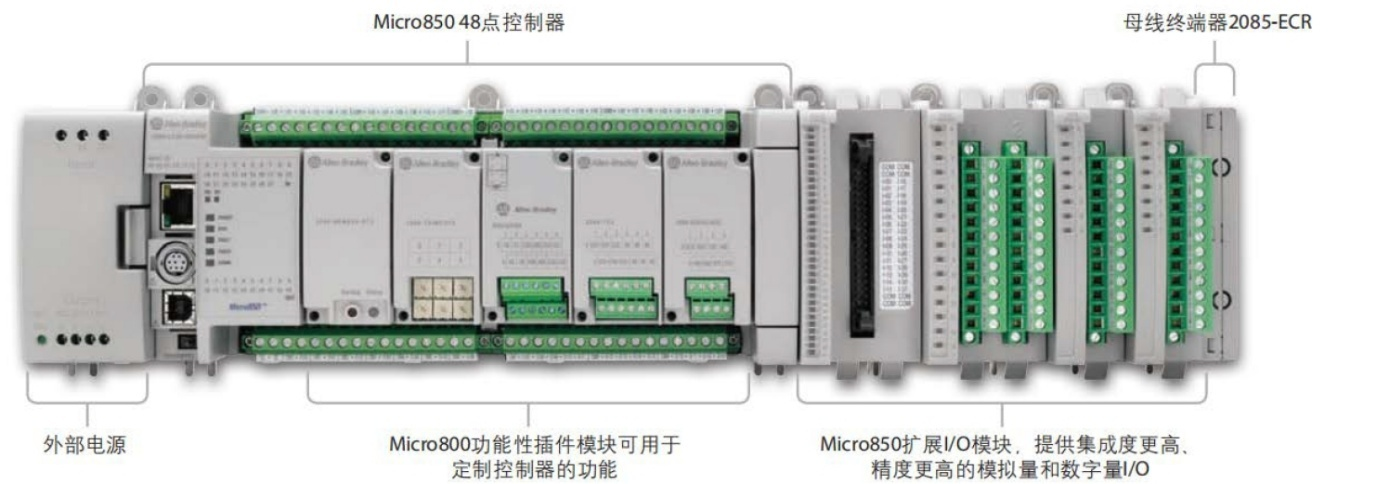
\includegraphics[width=0.9\linewidth]{image/Micro850控制器.png}
		\caption{Micro850控制器示意图}
		\label{chutian1}%文中引用该图片代号
	\end{minipage}
\end{figure}
\subsubsection{CCW编程软件与RSLinx通讯}
在本节课中，经由老师的讲解，我初步建立了对 CCW 编程软件的认知，掌握了基础开发流程，并对 RSLinx 通讯配置有了直观了解。\par
作为一款集设计与组态于一体的强大系统，CCW 不仅支持高效的程序逻辑编写，还集成了便捷的数据图像编辑与监控功能。在实际操作并将其与以往使用的 Visual Studio (VS) 等软件对比后，我深刻体会到了 CCW 在工业控制领域的独特优势，这些差异化的特性为我后续深入学习工控设计奠定了坚实基础。\par
相较于传统的通用编程工具，CCW 显著简化了工程开发难度，并提供了丰富的自定义配置：
\begin{itemize}
    \item 直观的交互布局：其界面设计高度符合工业逻辑，涵盖了从设备组态到通讯调试的完整菜单体系；工作区与工具箱的划分，让程序编写与模块监控变得触手可及。
    \item 梯形图 (LD) 的魅力：与 VS 依赖文本代码的模式不同，CCW 采用梯形图作为核心编程语言。这种图形化方式让逻辑结构一目了然，极大地降低了理解门槛。
    \item 高效的维护性：由于采用了功能块化的梯形图逻辑，程序的可读性得到了质的提升。在调整特定功能时，仅需针对相应的功能块进行修改，极大地提高了调试效率。
\end{itemize}

\begin{figure}[htbp]
	\centering
	\begin{minipage}{0.7\linewidth}
		\centering
		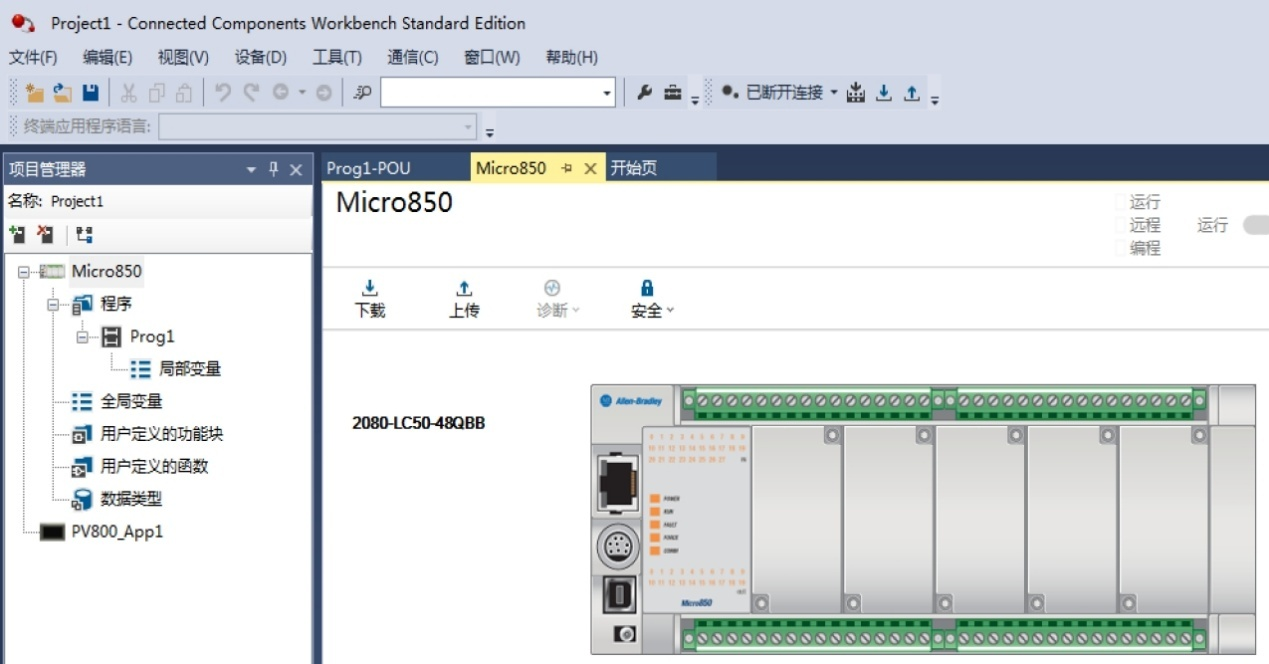
\includegraphics[width=0.9\linewidth]{image/CCW编程界面.png}
		\caption{CCW编程页面}
		\label{chutian1}%文中引用该图片代号
	\end{minipage}
\end{figure}

\subsubsection{基于PLC的数字量控制实验}
本节课通过编写两个具体程序，分别实现了利用 I-19、I-20 端子控制指示灯交替亮灭以及跑马灯循环的效果。\par
在两灯交替实验中，我们利用置位（Set）与复位（Reset）线圈构建逻辑。当触发 I-19 时，通过线圈驱动使 O-11 置 1、O-12 置 0；触发 I-20 时，逻辑反转使 O-12 置 1、O-11 置 0；而按下 I-21 则同时复位两个线圈。最终实现了：I-19 控制灯 11 亮、I-20 切换至灯 12 亮、I-21 实现全灭的控制目标。\par
第二个实验为跑马灯设计，核心在于利用 PLC 顺序执行的特性及 MOV 赋值模块。我们为八盏灯预设了 1 至 8 的编号，并配合比较、延迟和赋值模块编写逻辑。程序启动后，将变量 A1 设为 1，通过比较模块匹配后点亮 1 号灯；延时 500ms 后，利用赋值模块将变量更新为下一个编号，使前灯熄灭、后灯点亮。当循环至 8 号灯后，MOV 模块将变量重新复位为 1，从而实现往复循环。若按下 I-20 将变量强制清零，由于变量值与所有灯编号均不匹配，信号流随即终止，跑马灯停止运行。\par
通过本次实验，我对 CCW 编程有了更深体悟：首先，程序块的布局、信号流向与算法顺序至关重要，必须严格遵循逻辑规范以防报错。其次，在控制多元件间隔运动时，采用“单一变量关联多模块赋值”的思路非常高效，通过将不同元件映射至同一变量的不同状态值，可以极大地简化复杂系统的控制逻辑。
\begin{figure}[htbp]
	\centering
	\begin{minipage}{0.7\linewidth}
		\centering
		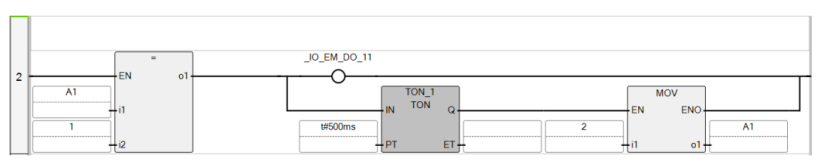
\includegraphics[width=0.9\linewidth]{image/跑马灯实验部分梯形图.png}
		\caption{跑马灯实验部分梯形图}
		\label{chutian1}%文中引用该图片代号
	\end{minipage}
\end{figure}

\subsubsection{PowerFlex变频器和丝杠运动控制实验}
本次实验的受控对象为滚珠丝杠，主要通过变频器实现对其手动与远程控制。滚珠丝杠的核心构造包括滚珠、螺纹套及螺纹导轨，其原理是利用滚珠在滚道内的滚动将旋转运动转化为线性运动。由于滚珠作为传动介质极大减小了摩擦阻力与轴向间隙，该机构具备极高的传动效率与定位精度。\par
在实验测试中，我们通过变频器向系统输入不同频率的信号。已知编码器每转脉冲数为 360，改变给定频率即可调节丝杠的线速度。尽管实际运行中存在微小偏差，但得益于丝杠结构对系统误差的抑制，脉冲当量基本稳定在 90 脉冲/mm 左右。\par
在程序编写方面，本次实验逻辑比之前的跑马灯更为简洁，重点在于掌握置位（Set）与复位（Reset）等新模块的应用。在实现不同功能时，必须准确配置局部变量以确保逻辑正确：例如，“启动”与“停止”功能应分别对应 start 和 stop 变量，而“正转”与“反转”则对应 FWD 和 REV。此外，丝杠行程计算的准确性至关重要。编码器将旋转反馈转化为脉冲数，这是实现精确位移控制的基础。在后续的三轴写字机实验中，若速度或行程计算失误，极易因超出物理限额而导致设备损坏。\par
最后，受控对象的物理保护不容忽视。在操作过程中，必须严密监控滑块位置，严禁滑块运动至两侧边缘触发限位开关，否则会导致变频器断电保护，影响实验连续性。同时，配置 PowerFlex 变频器参数时，需确保网络 IP 地址与本机网络环境严格匹配。这些细节不仅考验着操作的严谨性，更是保障实验顺利进行的必要前提。
\begin{figure}[htbp]
	\centering
	\begin{minipage}{0.7\linewidth}
		\centering
		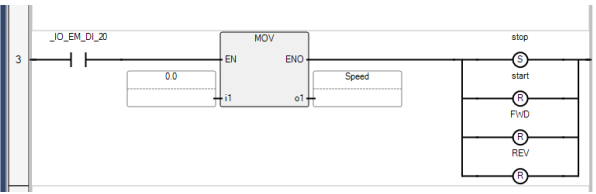
\includegraphics[width=0.9\linewidth]{image/丝竹杠实验部分梯形图.png}
		\caption{丝竹杠实验部分梯形图}
		\label{chutian1}%文中引用该图片代号
	\end{minipage}
\end{figure}

\subsubsection{基于PanelView触摸屏的PLC控制实验}
本次实验采用了分级控制架构：第一级为 PanelView 触摸屏人机界面，第二级为前述的滚珠丝杠等受控执行机构。在为期两周的课程中，我们首周完成了基于触摸屏的基础控制任务，次周则侧重于自主设计\textbf{多级分页管理界面}。\par
在首周实操中，我们成功实现了跑马灯、滚珠丝杠及同步带的分页控制。相比物理机柜的 I/O 硬件开关，触摸屏通过数字化按键提供了更直观的操作体验，显著优化了人机交互逻辑。进入第二周的自主设计阶段，我们通过在主界面布置“light”、“si\_gang”及“tong\_bu\_dai”等功能跳转按钮，实现了对三大核心任务的模块化管理。此外，通过配置“Goto Config”退出指令与“back”返回逻辑，使整体操作流更加清晰简洁。\par
通过本次实验，我们深入领悟了全局变量在 PLC 复杂组态中的核心枢纽作用。在初始设计阶段，由于错误配置了趋势图的输入变量类型，导致系统未达到预期显示效果。这一挫折让我们意识到，PLC 编程在数据类型严谨性上与 Python 等高级语言具有共通性。这种跨学科的经验提醒我们，在后续的工业控制程序开发中，必须对变量定义与类型匹配保持高度的职业严谨。
\begin{figure}[htbp]
	\centering
	\begin{subfigure}{0.49\linewidth}
		\centering
		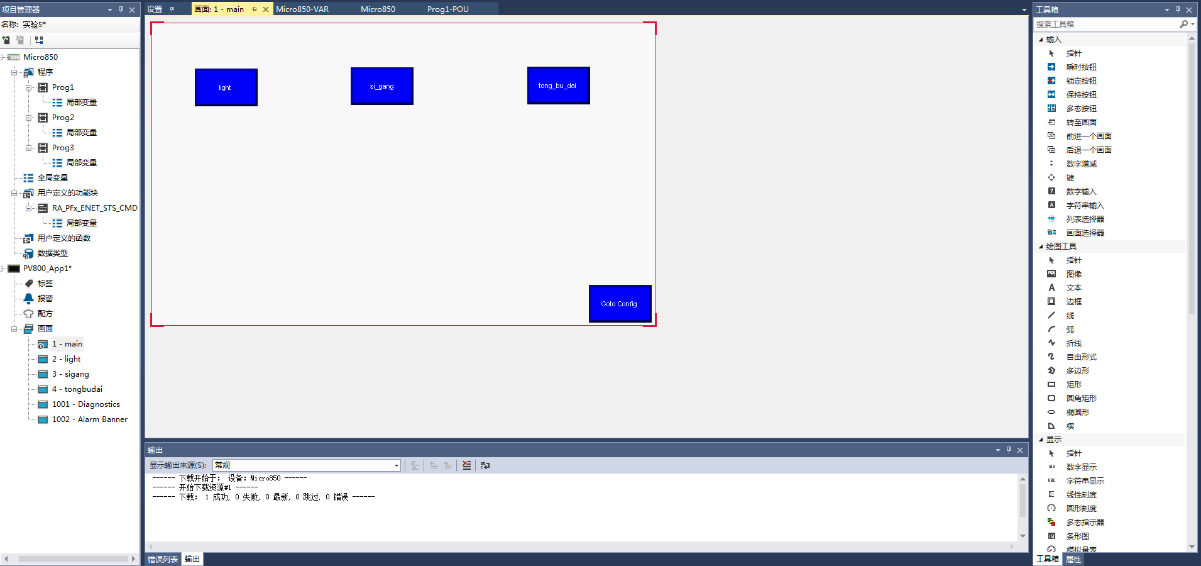
\includegraphics[width=0.9\linewidth]{image/panelview触摸屏设计.png}
		\caption{panelview触摸屏设计}
		\label{chutian3}%文中引用该图片代号
	\end{subfigure}
	\centering
	\begin{subfigure}{0.49\linewidth}
		\centering
		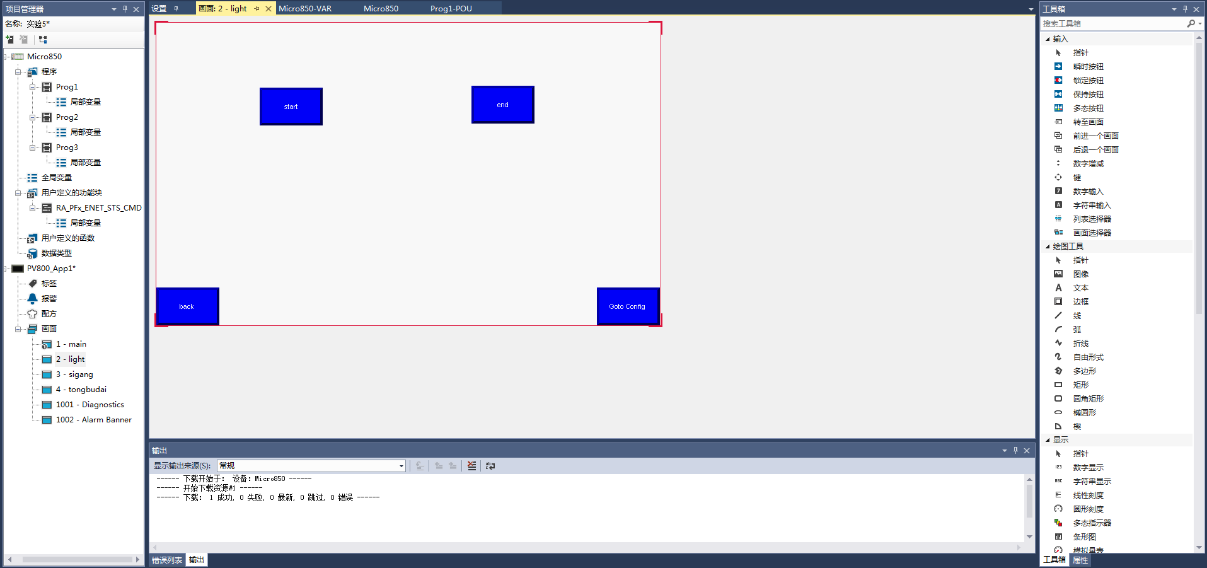
\includegraphics[width=0.9\linewidth]{image/跑马灯触摸屏设计.png}
		\caption{跑马灯触摸屏设计页面}
		\label{chutian4}%文中引用该图片代号
	\end{subfigure}
    \centering
	\begin{subfigure}{0.49\linewidth}
		\centering
		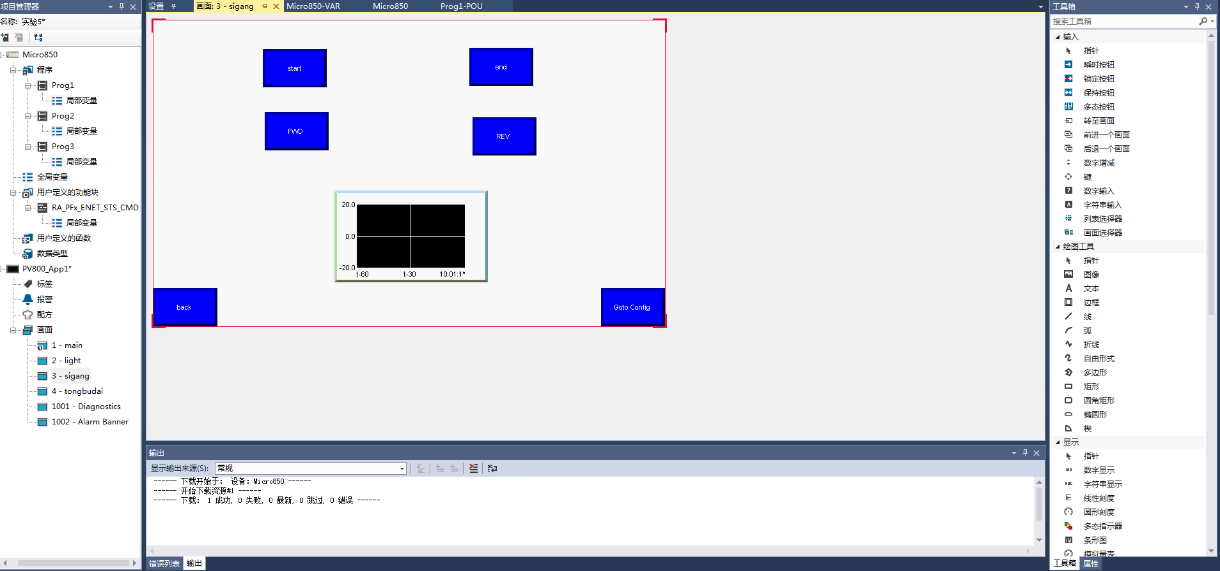
\includegraphics[width=0.9\linewidth]{image/滚竹丝杠触摸屏设计.png}
		\caption{滚竹丝杠触摸屏设计页面}
		\label{chutian5}%文中引用该图片代号
	\end{subfigure}
	\centering
	\begin{subfigure}{0.49\linewidth}
		\centering
		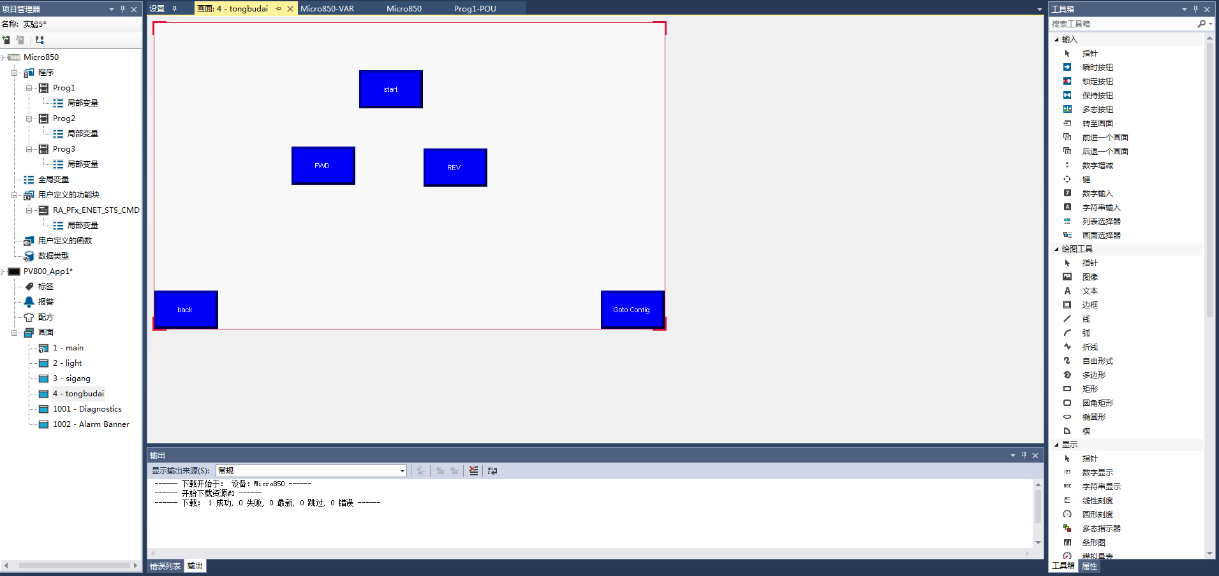
\includegraphics[width=0.9\linewidth]{image/同步带触摸屏设计.png}
		\caption{同步带触摸屏设计页面}
		\label{chutian6}%文中引用该图片代号
	\end{subfigure}
	\caption{PanelView触摸屏设计展示}
	\label{da_chutian}
\end{figure}

\subsubsection{同步带步进控制实验}
本次实验聚焦于同步带的双向步进控制系统。同步带传动依靠环形皮带内表面的等间距齿与带轮齿槽的精确啮合，实现运动与动力的可靠传递。系统的核心执行部件为步进电机，它负责将数字电脉冲信号精确转化为角位移或线位移，是现代数字化程序控制中的关键元件。\par
与侧重逻辑编程的跑马灯实验不同，本次实验的重心转向了运动轴的精密配置。我们必须预先设定同步带轴的关键参数，包括运行速度、电机额定转速及最高限速。配置过程需极度关注细节，例如若每转脉冲数的设定与驱动器物理细分不一致，将直接导致电机运行失准。完成轴配置后，通过特定功能块即可调用这些底层参数，进而实现在工控柜上对滑块双向相对运动的灵活操控。\par
在程序架构上，我们引入了运动控制功能块 MC\_MoveRelative，用于定义不同指令下的位移参数。具体逻辑设计如下：首先通过 MC\_Power 和 MC\_Reset 功能块实现电机的使能控制与故障清除；随后在核心梯级中使用 MC\_MoveRelative 设定正向与负向的相对运动增量。硬件交互方面，通过 I-19 按键触发系统上电，并由 I-20 与 I-21 分别下达正负向相对位移指令，从而完成了按键对同步带步进系统的全流程控制。

\subsubsection{基于PLC的三轴写字机运动控制实验}
本次的被控对象为三轴写字机。\par
本次实验分四周进行，第一周进行基于PLC的三轴写字机单轴运动控制实验，剩下三周进行三轴写字机的三周运动控制实验并设计轨迹。\par
三轴写字机器由三台步进电机驱动器驱动三台高扭矩步进电机，利用T型丝杆转动。T型丝杆刚性高、不容易形变，保证了写字的精度。\par
在第一周的实验中我们通过类似同步带控制中的相对运动模块实现对三轴写字机的运动控制，但是与同步带控制实验中不同，我们在此次实验设置了三根轴分别对应于三轴写字机的x、y、z轴。同样的，我们利用MC\_Power模块来分别对x、y、z轴进行上电，随后分别配置不同的Excute信号来进行轴的控制。最终实现了利用I-19来进行对三根轴的上电，利用I-20~I-25来分别实现控制x轴的正向前进，x轴的反向前进、y轴的正向前进，y轴的反向前进、z轴的正向前进，z轴的反向前进。\par
后三周实验过程中，我们完成了字的设计任务以及对于写字机的连贯控制任务，我们借助写字机完成了对于“科”的笔画书写，对于字体的设计图和写字机控制的最终实现效果如下图所示\par
\begin{figure}[htbp]
	\centering
	\begin{minipage}{0.48\linewidth}
		\centering
		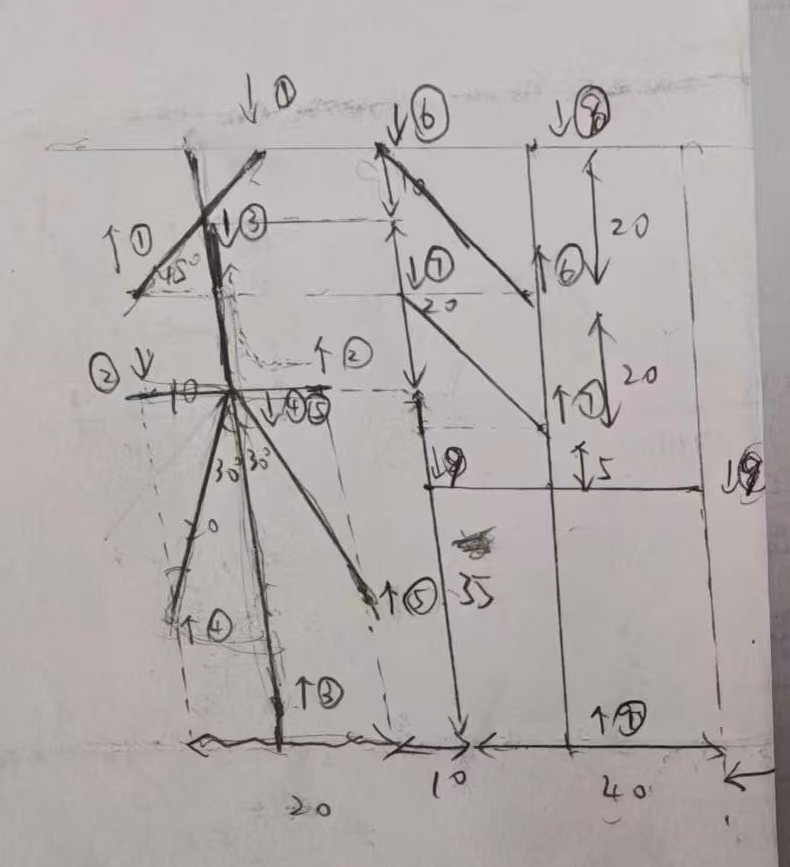
\includegraphics[width=0.9\linewidth]{image/三轴打字机设计草稿.png}
		\caption{三轴打字机写字草图设计}
		\label{chutian1}%文中引用该图片代号
	\end{minipage}
    \begin{minipage}{0.48\linewidth}
		\centering
		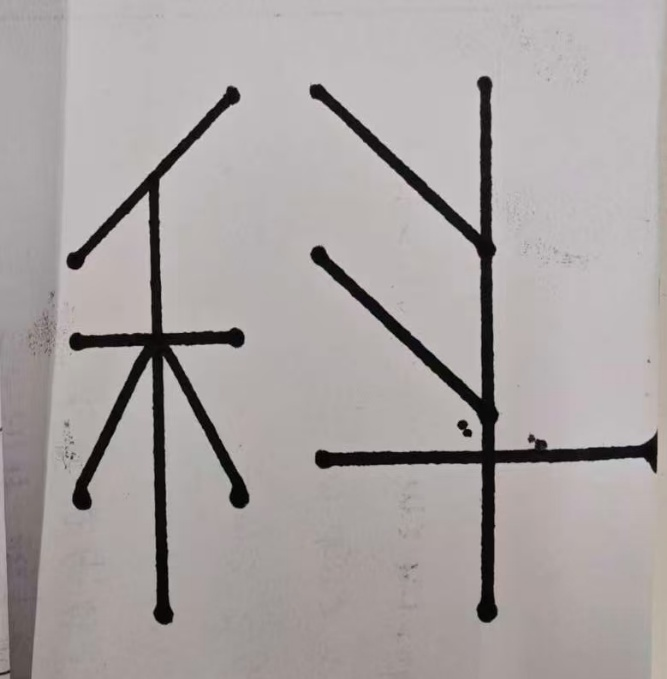
\includegraphics[width=0.9\linewidth]{image/三轴打字机写字机写字效果.png}
		\caption{三轴打字机最终写字效果}
		\label{chutian1}%文中引用该图片代号
	\end{minipage}
\end{figure}
实验过程中，我们也面临了运动规划与多轴同步的挑战。\par
在初始配置中，我们设定了单轴最大速度。然而，由于程序中运动时间设置不合理，导致指令要求的实际速度突破了硬件限制。这种偏差导致 xy 两轴无法同步起止：当两轴位移不等时，运动较快的一方会因限速而滞后，产生先“45度斜线”后“单轴横/纵向”的畸变轨迹。发现问题后，我们通过按比例设定三轴路径，确保理论上三轴能同时启停。\par
尽管建立了比例关系，但受限于电机误差及机械摩擦，三轴很难达到物理意义上的绝对同步。起初，我们利用 x 或 y 轴的完成信号作为笔画切换的标记，但这导致其他尚未复位的轴产生动作残余，造成指令执行的延迟。\par
为了攻克这一难题，我们将所有逻辑信号统一标定在 z轴 上。由于 z 轴负责起笔与落笔，将其作为程序运行的唯一判定基准，有效消除了时延现象。实测结果表明，输出效果最终与设计预期完美吻合。\par
本次实验不仅是对三轴写字机底层逻辑的深度解构，更是对复杂控制场景下权衡速度与精度的实战考验。通过对控制变量的综合优化，我不仅加深了对被控对象物理特性的理解，更在解决“理论模型”与“工程现实”差异的过程中，提升了严谨的逻辑设计能力。
\begin{figure}[htbp]
	\centering
	\begin{minipage}{0.7\linewidth}
		\centering
		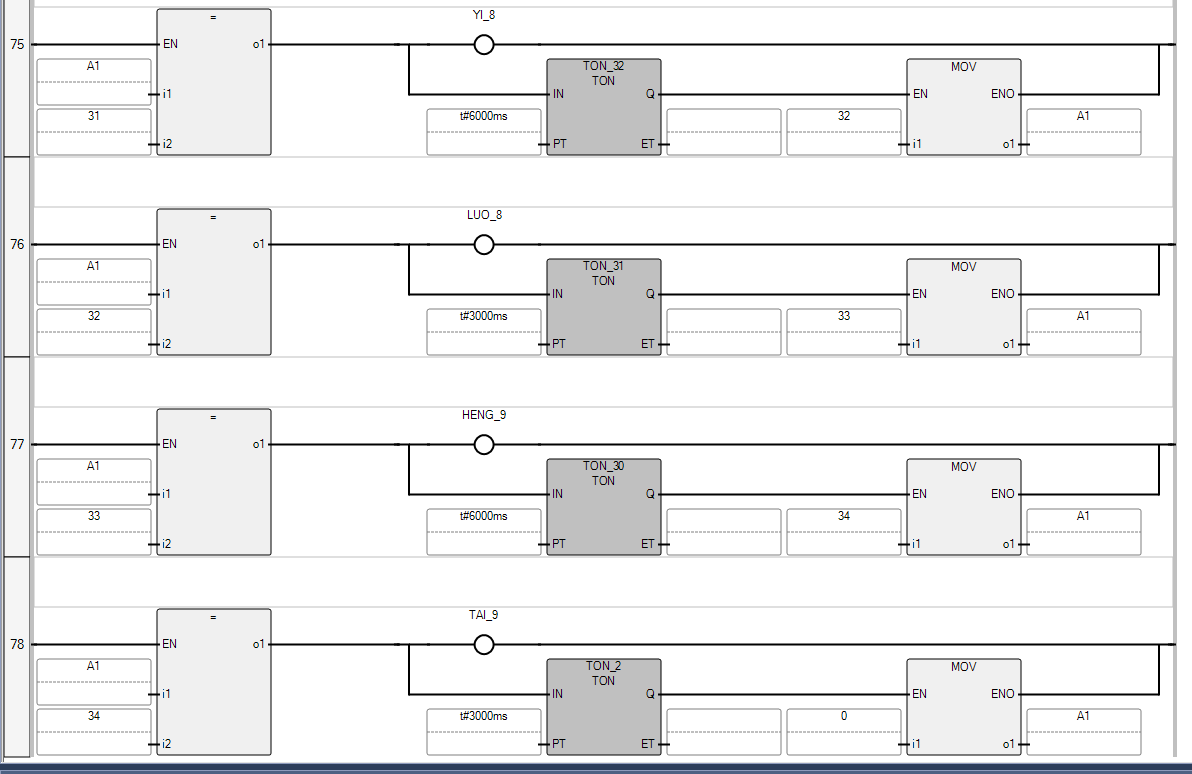
\includegraphics[width=0.9\linewidth]{image/三轴打字机实验部分梯形图.png}
		\caption{三轴打字机实验部分梯形图}
		\label{chutian1}%文中引用该图片代号
	\end{minipage}
\end{figure}
\subsubsection{基于PLC的小型手臂机器人运动控制实验}
\begin{figure}[htbp]
	\centering
	\begin{minipage}{0.7\linewidth}
		\centering
		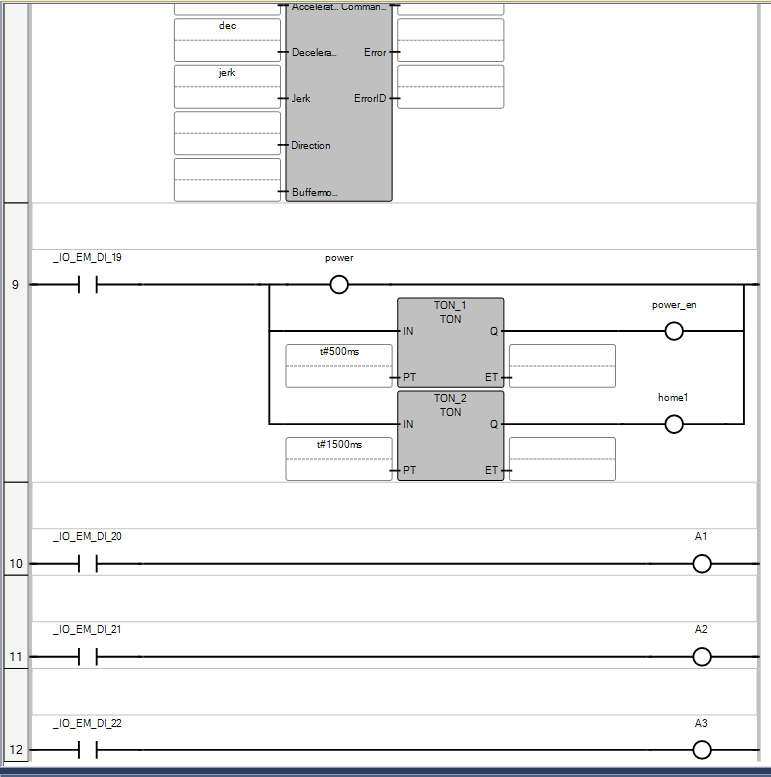
\includegraphics[width=0.9\linewidth]{image/小型手臂机器人部分实验梯形图.png}
		\caption{手臂机器人部分实验梯形图}
		\label{chutian1}%文中引用该图片代号
	\end{minipage}
\end{figure}
本次的被控对象为小型手臂机器人。\par
本堂课做的是基于PLC的小型手臂机器人三自由度运动控制实验,通过类似三轴写字机的运动控制，实现对于小型手臂机器人的运动控制。\par
在此次实验中我们采用了与之前实验不同的上电方式，我们设置了三个MC\_Power模块分别对三根轴进行使能。而后又利用三根轴的不同状态分别进行复位。当且仅当三根轴都成功上电之后我们才进行零位的标定。最后我们利用MC\_MoveAbsolute模块来控制手臂机器人的运动。\par
本次小型手臂机器人三自由度运动控制实验，通过对比之前三轴写字机控制方案，让我对 PLC 驱动多自由度设备的控制逻辑有了更细致的认知，尤其在设备使能、复位标定与精准定位环节，深刻体会到工业机器人控制中 “逻辑严谨性” 与 “操作规范性” 的核心要求。实验中采用三个独立 MC\_Power 模块分别对三轴使能，而非集中上电，这种设计不仅能精准判断单轴使能状态、便于故障排查，更契合工业场景中机器人模块化控制的思路 —— 工业机器人各轴负载、运动需求不同，独立使能可避免单轴故障影响整体设备运行，提升控制灵活性与可靠性。\par
“三轴均上电后才进行零位标定” 的操作逻辑，让我理解了工业机器人作业前 “初始化校验” 的重要性：零位是机器人精准定位的基准，只有确保各轴使能正常、复位到位，才能通过标定建立统一坐标体系，这与工业生产中机器人装配、搬运前的复位校准流程完全一致，可有效避免因定位偏差导致的作业误差或设备碰撞。而 MC\_MoveAbsolute 模块的应用，则直观展现了 PLC 在机器人绝对位置控制中的优势，对应工业场景中机器人精准抓取、定点放置等需求，体现了 “精准定位” 是工业机器人高效作业的核心保障。本次实验让我明白，多自由度机器人控制不仅是模块编程的简单组合，更需要围绕 “安全、精准、可靠” 的目标，设计合理的控制逻辑与操作流程，这为后续理解复杂工业机器人控制原理奠定了实践基础。\par
\subsubsection{基于PLC的小型手臂机器人协同控制实验}
本次实验的受控对象为多个三自由度小型机械臂。在基于 PLC 的运动控制基础上，我们通过以太网将前后两台机械臂进行物理连接，并采用主从协作控制模式，实现了主工控柜对两台设备的统一调度与管理。实验中，我组负责主程序的逻辑编写，通过选定特定的连接方案，与负责副程序的后续小组达成协同。\par
本次实操的关键在于首次应用了 MSG 通讯功能块。该模块是实现 PLC 间跨设备对话的核心，我们通过精准配置 MSG 模块中的目标 IP 地址，并配合 COP（复制）指令，成功实现了主副程序间的变量交互。为了确保数据在不同控制器间传输的稳定性与有效性，我们严格将相关交互变量定义为全局变量。\par
通过此次实验，我深入探究了 PLC 间的通讯逻辑及其在工业场景下的应用潜力，并对工厂自动化流水线的构建有了更清晰的构想。在实际生产中，利用多台 PLC 的通讯互联，以实时数据作为各工位的启停与运转信号，配合差异化的程序设计，即可实现流水线的有序联动。\par
同时，我也深刻意识到以太网交换机作为通讯媒介的重要性。它并非 PLC 系统的附属品，而是所有以太网通讯场景中的通用基础设施。在多设备协同控制体系中，交换机占据着核心地位，是保障多机械臂、多工位之间数据交换稳定与高效的关键基石。
\begin{figure}[htbp]
	\centering
	\begin{minipage}{0.49\linewidth}
		\centering
		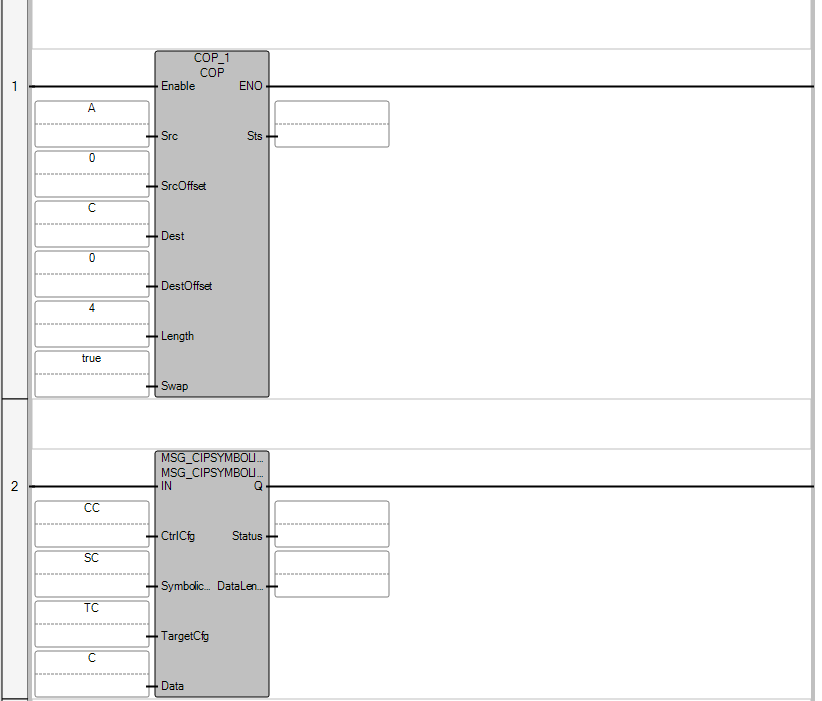
\includegraphics[width=0.9\linewidth]{image/手臂机器人梯形图.png}
		\caption{手臂机器人梯形图}
		\label{chutian1}%文中引用该图片代号
	\end{minipage}
	\centering
	\begin{minipage}{0.49\linewidth}
		\centering
		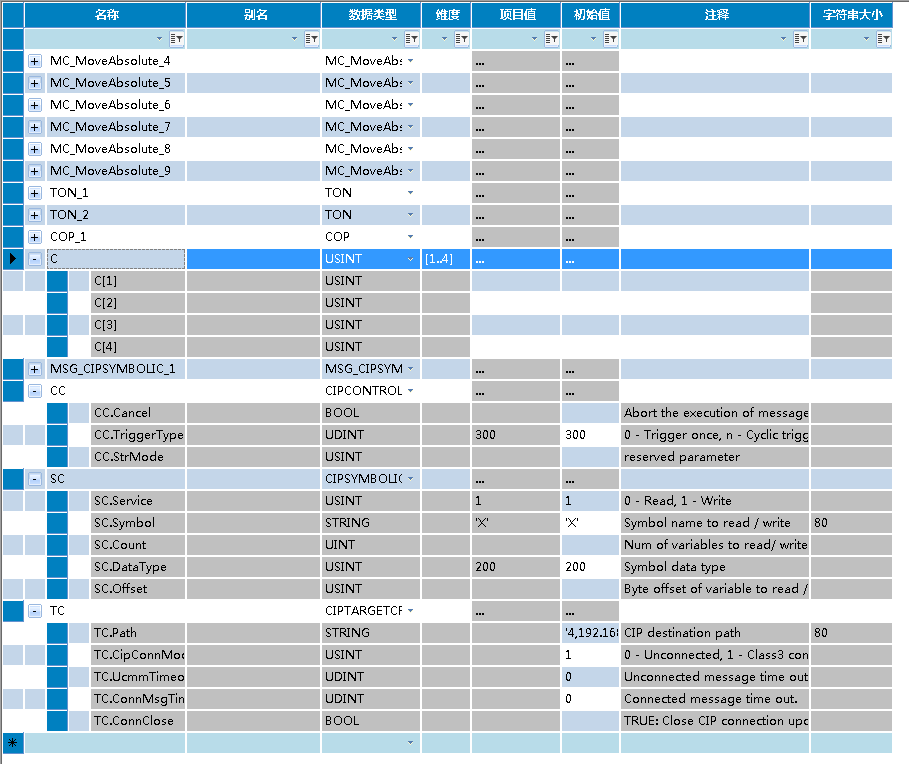
\includegraphics[width=0.9\linewidth]{image/手臂机器人变量图.png}
		\caption{手臂机器人变量图}
		\label{chutian1}%文中引用该图片代号
	\end{minipage}
\end{figure}
\subsection{课堂知识收获}
\subsubsection{工业控制系统及控制流程}
工业控制系统是将先进的控制技术与设备深度融合于生产流程的综合体系，其核心架构由硬件设备、软件系统及相关辅助设施共同支撑。\par
在硬件构成上，系统分为上位机与现场控制站两大层次。上位机多采用基于Windows与Intel架构的服务器或工作站，负责高层级的监控与管理。现场控制站则直接对接生产一线，核心部件包括执行运算与请求响应的中央处理单元（CPU）、连接现场设备的I/O输入输出模块、保障数据交互的通信接口，以及驱动整机运行的电源模块。此外，针对PID调节或温度监测等复杂工艺，还配有特定的智能功能模块。\par
软件体系则由上位机软件与现场控制站软件双重驱动。上位机部分涵盖了系统组态、实时控制、操作管理及网络诊断等应用软件；而现场控制站软件则具有高度的定制化特征，是由开发人员针对具体生产逻辑与工艺需求专门编写的程序。\par
根据生产模式的差异，控制系统可分为离散制造与流程工业两大类。离散制造系统以数字量检测为主，强调逻辑与顺序控制，其特点是信号实时性强、响应快，但由于常在室内环境运行，需重点防范电磁与粉尘干扰。流程工业系统则侧重于温度、压力、液位等模拟量的连续监测，多采用定值控制，其过程时间常数较大，由于生产现场往往处于室外，对设备的防水、防爆及本质安全性能有着更严格的要求。
\subsubsection{各类被控对象的运动控制}
以下列举本课程中使用过的各种被控对象:\par
\begin{enumerate}
\item \textbf{滚珠丝杠}:\par
\qquad 滚珠丝杠是一种精密的机械传动元件。丝杠上具有精细的螺纹，滚珠在丝杠的螺纹槽内滚动，通过滚珠的循环运动，能够实现转动与直线运动的相互转化\par
它具有许多优点，包括高精度、低阻力、高效率和可逆性。这主要是因为滚珠丝杠利用了滚动摩擦代替滑动摩擦，使得其能够在较低的驱动力下运行并提供非常精确的运动控制，因此被广泛应用于数控机床、3D打印机、自动化设备等领域\par
其关键部件组成是：螺杆（带螺纹的长杆）、螺母（内部有与螺杆匹配的螺纹）、钢球（在螺杆和螺母之间的滚道上滚动）、预压片（调整滚珠丝杠的预紧力）、反向器（改变钢球的方向）和防尘器（保护滚珠丝杠免受灰尘和其他污染物的影响）。这些组件在制造过程中需要进行精细的加工和组装，以保证滚珠丝杠的高精度性能。
\item \textbf{同步带}:\par
\qquad 同步带是一种用于精确传输动力的机械装置。它由带体和齿轮组成，带体通常由橡胶、聚氨酯等材料制成，齿轮则与带体的齿形相配合。当驱动轮转动时，通过摩擦力将动力传递给同步带上，然后带动从动轮一起旋转。由于同步带的齿形与带轮完全啮合，能够有效地避免打滑现象，确保运动的精确传递和低噪音运行。同步带广泛应用于各种机械设备中，如数控机床、包装设备、打印机等\par
\qquad 步进电机则是一种能够将电脉冲信号转换为相应角位移或线位移的电动机。每输入一个脉冲信号，步进电机就会转动一定的角度或前进一步，其输出的角位移或线位移与输入的脉冲数成正比。这种特性使得步进电机非常适合于需要精确位置控制的应用，例如在机器人、3D打印、医疗设备和自动贩卖机等领域\par
\qquad 两者合作可以实现精准、高效的动力传输和运动控制，在不同的自动化应用中扮演着重要的角色。
\item \textbf{三轴写字机}:\par
\qquad 三轴写字机是一种用于精确书写或绘画的自动化设备。它通常由三个运动轴（X、Y、Z轴）组成，每个轴通过电机驱动，并通过丝杠或同步带传动机构实现精确的位置控制。在三轴写字机的一个重要部件是固定在Z轴上的笔或绘图工具。根据输入的计算机程序，三轴平台按照预定路径进行移动，使得笔能够在纸张或其他材料上完成复杂的书写或绘图工作。控制三轴写字机通常配备专门的控制软件，用户可以通过计算机程序或触摸屏界面进行编程，设定参数、导入所需的文本或图案，由写字机自动完成书写或绘制任务\par
\qquad 由于其高精度、灵活性和可重复性，三轴写字机被广泛应用于教育科研、艺术创作和工业设计。由于技术的进步和普及，三轴写字机也越来越受到手工艺者和设计师的青睐。
\item \textbf{小型手臂机器人}:\par
\qquad 小型手臂机器人是一种用于自动化处理和装配任务的设备。它通常由多个关节和驱动电机组成，每个关节通过电机驱动，并通过精确的位置控制实现运动。这些关节赋予手臂多个自由度，使其可以在三维空间中进行复杂的动作。小型手臂机器人根据特定的应用需求可以配备不同的末端执行器，如夹持器、吸盘、焊接工具等，以便实现预期功能。它们通常被编程来执行重复性的任务，如组装电子产品、包装和质量检查，从而大幅提高生产效率，同时有效避免人工操作可能导致的错误\par
\qquad 小型手臂机器人以其灵活性、精确性和适应性在现代自动化和智能化的进程中发挥着越来越重要的作用，应用范围涵盖工业生产、医疗、教育培训、物流等多个领域。由于其紧凑的设计和灵活性，它们尤其适合于空间有限或者需要高精度操作的任务环境。

\end{enumerate}
\subsubsection{工业PLC控制系统}
工业PLC控制系统是以可编程逻辑控制器为核心的自动化架构，旨在工业生产中实现高效的监测与调节。该系统利用可编程存储器存储各类逻辑、顺序、定时、计数及算术运算指令，通过数字或模拟信号的输入输出，指挥机械设备完成特定的工艺流程。其设计准则强调与工业系统的无缝集成，并具备良好的功能扩展性。\par
PLC的工作机制采用循环扫描模式，每个周期包含输入采样、程序执行和输出刷新三个阶段。在采样阶段，PLC将外部输入的状态存入I/O映像区；随后在执行阶段，CPU按顺序扫描并计算用户程序；最后在刷新阶段，根据运算结果更新输出锁存电路，进而驱动外围设备。由于这种循环机制对突发信号的响应存在延迟，部分高性能PLC引入了中断处理机制以提升实时性。\par
在实际应用中，PLC的功能涵盖了多个维度：首先是逻辑控制，广泛应用于电梯、包装线等自动化流水线的开关量调度；其次是运动控制，通过精密模块驱动伺服或步进电机实现定位；再者是过程控制，用于调节温度、压力及流量等连续变化的物理量；最后是数据处理，能够完成复杂的数学运算、数据转换与逻辑排序，满足智能化生产的需求。

\section{感想与认识}

\subsection{介绍一种自己所了解的工业自动化控制系统}
分布式控制系统（DCS）是现代大型工业流程自动化的核心中枢，其设计哲学的精髓在于“分散控制，集中管理”。不同于早期的集中式控制系统将风险高度集中，DCS 通过一种层级化的架构，将具体的控制任务下放到分散在现场的各个控制器中，而将监视、操作和管理的权限集中在中央控制室。这种架构既保证了生产现场的风险分散与控制的实时性，又赋予了操作人员对整个工厂宏观、统一的调度能力，是化工、电力、冶金等连续性生产行业不可或缺的基础设施。\par

DCS 的硬件架构并非简单的设备堆砌，而是一个由下至上紧密协作的有机整体。在物理层的最前端，\textbf{输入/输出模块（I/O）} 充当着系统的感官，负责采集现场传感器的数据并驱动执行机构；这些信号随即被传输至 \textbf{现场控制站（FCS）}，这是系统的“大脑”，内部运行着微处理器，负责独立执行 PID 调节、逻辑运算等具体的控制策略，且互不干扰。为了实现人与系统的交互，\textbf{操作员站（OS）} 提供了可视化的窗口，操作人员在此通过图形界面监视全厂状态并下达指令；而 \textbf{工程师站（ES）} 则专供专业人员进行系统的组态、编程与维护。连接这一切的“神经系统”是多层级的 通信网络，它承载着从现场实时数据到上层管理信息的高速流动，确保了各个孤立的单元能够协同工作，构成一个完整的自动化系统。\par

DCS 最为显著的特点在于其极致的 \textbf{高可靠性与冗余设计}。为了适应连续生产对稳定性的严苛要求，DCS 的关键部件——如控制器、电源模块及通信网络——通常都采用 1:1 的热备冗余配置，一旦主设备发生故障，备用设备能在毫秒级时间内无缝接管，确保生产过程不受任何干扰。此外，DCS 具备强大的 开放性与算法丰富性，它不仅内置了诸如串级、前馈、解耦等复杂的控制算法库，能够轻松应对非线性、大滞后的模拟量控制需求，还支持各类标准通信协议，能够灵活地与第三方设备或上层的 MES、ERP 管理系统进行数据交互，打破了信息孤岛。同时，其 易于扩展 的特性使得工厂可以随着产能的增加，随时平滑地增加控制节点而不必推翻原有系统。\par

在实际应用中，DCS 的优势主要体现为\textbf{对大规模、高风险流程的 卓越掌控力与安全性}。由于控制风险被分散到了无数个独立的控制器中，局部故障绝不会扩散导致全厂瘫痪，这对于一旦停机就会造成巨大经济损失甚至安全事故的流程工业至关重要。其次，DCS 极大地提升了 管理效率与维护便捷性，它能够处理数以万计的 I/O 点，将海量的生产数据转化为直观的趋势图和报警信息，让操作员能够“决胜千里之外”；同时，其支持“热插拔”的维护方式，允许技术人员在系统带电运行的情况下更换故障模块，真正实现了生产过程的连续性与设备维护的灵活性的完美统一。


\subsection{课程感想}
过本学期智能工业控制系统实践课程的学习，我收获颇丰。从最初对工业控制系统的陌生，到现在能够熟练使用CCW软件进行PLC编程，能够控制滚珠丝杠、同步带、三轴写字机、小型手臂机器人等多种被控对象，这一路的学习让我对工业自动化有了全新的认识。\par
在理论层面，我深入理解了工业智能与通用人工智能的本质区别：工业智能强调强物理关联性、极高的稳定性与安全性要求、严格的实时性与确定性，这些特点决定了工业控制系统必须采用与通用AI不同的设计理念和实现方式。\par
在实践层面，我掌握了CCW梯形图编程的基本方法，学会了如何配置运动轴参数、如何使用各种功能块（如MC\_Power、MC\_MoveRelative、MC\_MoveAbsolute、MSG等）来实现复杂的控制逻辑。特别是在三轴写字机轨迹设计实验中，我深刻体会到了多轴协同控制的复杂性，以及如何通过合理的程序设计来解决实际问题。\par
在团队协作层面，小型手臂机器人协同控制实验让我认识到了PLC间通讯的重要性，也让我对工厂流水线的实现有了更直观的理解。通过多台PLC间的通讯连接，以数据传递作为设备启停、运转的控制信号，就能实现流水线各环节的有序联动。\par
综合上述内容，这门课程不仅让我学到了工业控制的专业知识，更重要的是培养了我的工程思维和实践能力。我相信这些知识和能力将在我未来的学习和工作中发挥重要作用。

\end{document}